\documentclass[12pt,a4paper]{article}

%------------------------------------------------
% Packages
%------------------------------------------------
\usepackage[margin=1in]{geometry}
\usepackage{setspace}
\usepackage{lmodern}
\usepackage[T1]{fontenc}
\usepackage{microtype}
\usepackage{xcolor}
\usepackage{graphicx}
\usepackage{enumitem}
\usepackage{titlesec}
\usepackage{ragged2e}
\usepackage{parskip} % no paragraph indent, adds space
\usepackage{caption}
\usepackage{fancyhdr}
\usepackage{listings}
\lstset{
    language=Python,
    basicstyle=\ttfamily\small,
    keywordstyle=\color{blue},
    stringstyle=\color{brown},
    commentstyle=\color{teal},
    showstringspaces=false,
    breaklines=true,
    frame=single,
    numbers=left,
    numberstyle=\tiny,
    xleftmargin=2em,
    framexleftmargin=1.5em
}

%------------------------------------------------
% Colors and styles
%------------------------------------------------
\definecolor{sectionbar}{HTML}{E9A640} % orange bar color similar to the image
\definecolor{sectiontext}{HTML}{2B2B2B}

% Wide, colored bar style for "section-like" headers
\newcommand{\sectionbar}[1]{%
  \vspace{0.6\baselineskip}%
  \noindent
  \colorbox{sectionbar}{%
    \parbox{\dimexpr\linewidth-2\fboxsep\relax}{%
      \textbf{\Large\textsf{#1}}%
    }%
  }%
  \vspace{0.6\baselineskip}
}

% Body text tweaks
\setstretch{1.2}
\setlist[itemize]{leftmargin=1.2em}
\setlist[enumerate]{leftmargin=1.2em}

% Section title spacing (not used directly since we use custom bars)
\titlespacing*{\section}{0pt}{1ex}{0.6ex}

% Figure captions smaller and tight
\captionsetup{font=small,labelfont=bf}

% Footer with page number
\pagestyle{fancy}
\fancyhf{}
\cfoot{\thepage}

%------------------------------------------------
\begin{document}

%================================================
% LABORATORY SESSION 1
%================================================
\sectionbar{LABORATORY SESSION 1}

%---------------- INTRODUCTION -------------------
\sectionbar{INTRODUCTION}

\justifying
The aim of the laboratory session was to provide gain a hands-on experience on how different algorithms like Myers and Histogram behave on real-world open source repositories. It also made us explore difference between code artifacts and non-code artifacts in the context of software development. It also aims to make us understand the difference in comparisons when the code ignores whitespace and blank lines. Importantly, how discrepancies can highlight the strengths of diff algorithms. After the lab, we aim to be proficient in analyzing diff outputs, generate datasets, visualize mismatches using python plots.

%---------------- SETUP --------------------------
\sectionbar{SETUP}

\begin{itemize}
    \item \textbf{Software and Tools Used:}
    \begin{itemize}
        \item Operating System: macOS
        \item Text Editor: Visual Studio Code
        \item Version Control: git
        \item Remote Hosting: GitHub
        \item Continuous Integration: GitHub Actions
    \end{itemize}
    \item \textbf{Repositories:}
    \begin{itemize}
        \item \texttt{butterknife} -- A popular view binding library for Android that helps reduce boilerplate code when working with UI components. 
        \item \texttt{retrofit} -- A type-safe HTTP client for Android and Java, widely used for making API requests and handling network operations.
        \item \texttt{glide} -- An image loading and caching library for Android, optimized for smooth scrolling and efficient resource usage.
    \end{itemize}
    \item \textbf{Python Libraries:}
    \begin{itemize}
        \item Pydriller: A Python framework for mining software repositories. Used to analyze git repositories and extract commit information.
        \item Pandas: To manage dataframes and dealing with CSV files
    \end{itemize}
    \item \textbf{Initial Steps:}
    \begin{itemize}
        \item GitHub account: TejasLohia21
        \item SSH key configured for secure push/pull
        \item Virtual Environment named lab4 to manage library versions
        \item Configured git username and email
        \item Cloned/initialized three repository
    \end{itemize}
\end{itemize}

%------------- METHODOLOGY AND EXECUTION ---------
\sectionbar{METHODOLOGY AND EXECUTION}

\subsection*{Part A: Repository selection}
\begin{itemize}
        \item \texttt{butterknife} -- A popular view binding library for Android that helps reduce boilerplate code when working with UI components. 
        \item \texttt{retrofit} -- A type-safe HTTP client for Android and Java, widely used for making API requests and handling network operations.
        \item \texttt{glide} -- An image loading and caching library for Android, optimized for smooth scrolling and efficient resource usage.
    \end{itemize}

\subsection*{Part B: Adding README File and Pushing Changes}

Repositories were chosen using the criterias which were mentioned in lectures and in the assignment:
\begin{itemize}
    % \item \texttt{fastapi} -- A modern, high-performance web framework for building APIs with Python.
    %     \begin{itemize}
    %         \item \textbf{Commits:} The repository has 5790 commits, which is in the range of $[1206,\ 25000]$.
    %         \item \textbf{Stars:} The repository has 88.9k stars, making it a real and highly used project.
    %         \item 
    %     \end{itemize}
    \item \texttt{butterknife} -- A popular view binding library for Android that helps reduce boilerplate code when working with UI components.  
        \begin{itemize}
            \item \textbf{Commits:} The repository has 1016 commits, which is within the acceptable range for analysis.
            \item \textbf{Stars:} The repository has 28.8k stars, indicating strong community usage and real-world relevance.  
            \item \textbf{Myers Algorithm:} Since Git uses Myers as the default diff algorithm, we can directly apply \texttt{git diff --diff-algorithm=myers} on Butterknife.  
            \item \textbf{Histogram Algorithm:} Git also supports the Histogram algorithm, which works with the Butterknife repository using \texttt{git diff --diff-algorithm=histogram}.  
            \item \textbf{Discrepancy Analysis:} With over a thousand commits and frequent UI-related code changes, Butterknife provides meaningful opportunities to compare Myers and Histogram diffs.  
            \item \textbf{Required Files:} The repository includes \texttt{butterknife/} source code, a dedicated \texttt{tests/} suite, along with \texttt{README.md} and \texttt{LICENSE}, thus satisfying all the required file-type conditions.  
            \item \textbf{Conclusion:} Butterknife is one of the academically researched repositories for discrepancy analysis in both the Myers and Histogram algorithms.
        \end{itemize}
    \item \texttt{requests} -- A popular Python library for making HTTP requests in a simple and human-friendly way.
        \begin{itemize}
            \item \textbf{Commits:} The repository has 6372 commits, which is in the range of $[1206,\ 25000]$.
            \item \textbf{Stars:} The repository has 53.2k stars, showing that it is widely used and well-established.
            \item \textbf{Myers Algorithm:} Since Git uses Myers as the default diff algorithm, we can directly apply \texttt{git diff --diff-algorithm=myers} on the Requests repository.
            \item \textbf{Histogram Algorithm:} Git also supports the Histogram algorithm, which works with this repository using \texttt{git diff --diff-algorithm=histogram}.
            \item \textbf{Discrepancy Analysis:} With thousands of commits and frequent code updates, the Requests repository provides sufficient changes to compare Myers and Histogram diffs effectively.
            \item \textbf{Required Files:} The repository contains the \texttt{requests/} source directory, a large \texttt{tests/} suite, along with \texttt{README.md} and \texttt{LICENSE}, fulfilling the file-type requirements.
        \end{itemize}
    \item \texttt{glide} -- A fast and efficient image loading and caching library for Android, widely used for handling media in mobile applications.  
        \begin{itemize}
            \item \textbf{Commits:} The repository has 3047 commits, which lies in the range of $[1206,\ 25000]$, making it suitable for analysis.  
            \item \textbf{Stars:} The repository has 34.9k stars, showing its strong adoption and relevance in real-world projects.  
            \item \textbf{Myers Algorithm:} Since Git uses Myers as the default diff algorithm, we can directly apply \texttt{git diff --diff-algorithm=myers} on the Glide repository.  
            \item \textbf{Histogram Algorithm:} Git also supports the Histogram algorithm, which works seamlessly with this repository using \texttt{git diff --diff-algorithm=histogram}.  
            \item \textbf{Discrepancy Analysis:} With over three thousand commits and consistent updates, the Glide repository provides enough modifications to effectively compare Myers and Histogram diffs.  
            \item \textbf{Required Files:} The repository includes the \texttt{glide/} source code, a dedicated \texttt{tests/} suite, along with \texttt{README.md} and \texttt{LICENSE}, satisfying the file-type requirements.  
        \end{itemize}
\end{itemize}
\newpage

\subsection*{Part C: Run Software Tool on the Selected Repository:}
\begin{figure}[h!]
    \centering
    \includegraphics[width=0.8\textwidth]{/Users/tejasmacipad/Downloads/WhatsApp Image 2025-08-30 at 15.52.26.jpeg}
    \caption{Central Code to extract diff.}
    \label{fig:diff-example}
\end{figure}

\begin{lstlisting}[language=Python, caption={Diff analysis script for selected repositories}]
import csv
import re
import os
import subprocess
from pydriller import Repository
from git import Repo

local_repo_paths = [
    "/Users/tejasmacipad/Desktop/Third_year/STT/lab4/butterknife",
    "/Users/tejasmacipad/Desktop/Third_year/STT/lab4/retrofit",
    "/Users/tejasmacipad/Desktop/Third_year/STT/lab4/glide"
]
output_csv_filename = "diff_analysis_results.csv"

csv_header = [
    "repository_name", "old_file_path", "new_file_path", "commit_SHA",
    "parent_commit_SHA", "commit_message", "diff_myers", "diff_hist", "Discrepancy"
]

with open(output_csv_filename, 'w', newline='', encoding='utf-8') as csvfile:
    csv_writer = csv.writer(csvfile)
    csv_writer.writerow(csv_header)

    five_mb = 5 * 1024 * 1024
    printat = five_mb

    for path in local_repo_paths:
        print(f"Processing repository: {os.path.basename(path)}")

        try:
            for commit in Repository(path).traverse_commits():
                if not commit.parents:
                    continue

                parent_sha = commit.parents[0]

                for mod in commit.modified_files:
                    if mod.filename.endswith(('.png', '.jpg', '.jpeg', '.gif', '.zip')):
                        continue

                    filepathdiff = mod.new_path or mod.old_path
                    if not filepathdiff:
                        continue

                    common_args = ["git", "-C", path, "diff", parent_sha, commit.hash, "--", filepathdiff]

                    myers_proc = subprocess.run(common_args, capture_output=True, text=True, encoding='utf-8', errors='ignore')
                    hist_proc = subprocess.run(common_args + ["--diff-algorithm=histogram"], capture_output=True, text=True, encoding='utf-8', errors='ignore')

                    myers_diff_text = myers_proc.stdout
                    hist_diff_text = hist_proc.stdout

                    norm_myers = "\n".join([re.sub(r'\s+', '', line) for line in myers_diff_text.splitlines() if re.sub(r'\s+', '', line)])
                    norm_hist = "\n".join([re.sub(r'\s+', '', line) for line in hist_diff_text.splitlines() if re.sub(r'\s+', '', line)])

                    discrepancy_found = "Yes" if norm_myers != norm_hist else "No"

                    csv_writer.writerow([
                        os.path.basename(path), mod.old_path, mod.new_path,
                        commit.hash, parent_sha, commit.msg,
                        myers_diff_text, hist_diff_text, discrepancy_found
                    ])

                    current_size = os.path.getsize(output_csv_filename)
                    if current_size >= printat:
                        size_in_mb = current_size / (1024 * 1024)
                        print(f"--> CSV file size has reached {size_in_mb:.2f} MB.")
                        printat += five_mb

        except Exception as error:
            print(f"An error  processing {os.path.basename(path)}: {error}")
            continue

print(f"\nAnalysis finished. Results are in {output_csv_filename}")
\end{lstlisting}

\subsection*{Explanation of the Code}

The code shown in Figure~\ref{fig:diff-example} is responsible for extracting the differences between file versions in the selected repositories. It leverages the Pydriller library to iterate through each commit and retrieve the modified files. For each file, the code applies both the Myers and Histogram diff algorithms using Git commands, capturing the output for further analysis.

Key steps in the code:
\begin{itemize}
    \item Store all the paths to the repositories in \texttt{local\_repo\_paths}.
    \item Define the output csv\_filename and also define the csv\_header for that csv file which contains all the columns asked in the part (c) of the assignment.
    \item Algorithm then starts iterating through each repository path, ans also tracks the size of growing csv file.
    \item Iterating through every commit of that repository which initially fetches the hash value of the commmit.
    \item Extraction of parent\_sha (We only take the first parent in case of a merge commit). Following this, we iterate through each of the modified files in that commit.
    \item Defining \texttt{common\_args} which stores commands to be passed on to the \texttt{subprocess.run()} as arguments.
    \item We obtain the Myers diff and Histogram diff outputs by executing the respective Git commands and capturing their output and apply normalization
    \item Defining discrepancy\_found if the outputs of the two algorithms differ and commit the output to the CSV file
\end{itemize}

This approach allows for systematic extraction and comparison of diff outputs, facilitating the analysis of discrepancies between the Myers and Histogram algorithms across real-world code changes.

\subsection*{Part D: Compare Diff Outputs for Discrepancy Analysis}

After processing all the repositories we record the output of both the algorithms (Myers and Histogram) in a CSV file.

\begin{enumerate}
    \item \textbf{Normalization:}  
    To ensure fairness in comparison, whitespace and blank lines were ignored.

    \item \textbf{Comparison Logic:}  
    The normalized Myers output and Histogram output were compared line by line.  
    \begin{itemize}
        \item If both were identical, the entry was labeled \texttt{No} discrepancy.  
        \item If they differed, the entry was labeled \texttt{Yes} discrepancy.  
    \end{itemize}

    \item \textbf{CSV Output:}  
    A dedicated column named \texttt{Discrepancy} was added to the CSV file. This column stores either \texttt{Yes} or \texttt{No} for each commit-file pair.

\end{enumerate}

\subsection*{Part E: Final Dataset Statistics and Exploratory Analysis}

\begin{figure}[h!]
    \centering
    \includegraphics[width=0.8\textwidth]{/Users/tejasmacipad/Downloads/WhatsApp Image 2025-08-30 at 17.23.55.jpeg}
    \caption{Central Code to extract diff.}
    \label{fig:diff-example}
\end{figure}

After collecting and storing the diff results from all three repositories, we performed an exploratory analysis of the final dataset. The analysis focused on quantifying discrepancies and categorizing them based on file types.

\begin{enumerate}
    \item \textbf{File Categorization:}  
    Each modified file was categorized into one of the following groups: 
    \textit{Source code}, \textit{Test code}, \textit{README}, \textit{LICENSE}, or \textit{Other}.  
    This categorization was performed by checking the file extensions and naming patterns (e.g., files containing ``test'' were labeled as Test code).

    \item \textbf{Mismatch Detection by Category:}  
    For each category, the total number of files and the number of files with discrepancies between the Myers and Histogram algorithms were computed. This enabled us to analyze which file types were more prone to mismatches.

    \item \textbf{Statistical Summary:}  
    The following statistics were derived from the analysis:
    \begin{itemize}
        \item Total files analyzed across all repositories: \textbf{31,344}.  
        \item Overall mismatches detected: \textbf{1,108}, corresponding to approximately \textbf{3.54\%} of the total files.  
        \item Breakdown of mismatches by file category:  
        \begin{itemize}
            \item \textbf{Source code:} 14,515 files, 616 mismatches (\textbf{4.24\%}).  
            \item \textbf{Test code:} 9,282 files, 428 mismatches (\textbf{4.61\%}).  
            \item \textbf{README files:} 381 files, 12 mismatches (\textbf{3.15\%}).  
            \item \textbf{LICENSE files:} 17 files, 0 mismatches (\textbf{0\%}).  
            \item \textbf{Other files:} 7,149 files, 52 mismatches (\textbf{0.73\%}).  
        \end{itemize}

        \item \textbf{File Extension Summary (Top 10):}  
            \begin{itemize}
                \item \textbf{.java:} 23,281 files, 1,040 mismatches (4.47\%)  
                \item \textbf{.kt:} 350 files, 14 mismatches (4.00\%)  
                \item \textbf{.md:} 541 files, 15 mismatches (2.77\%)  
                \item \textbf{Other:} 142 files, 3 mismatches (2.11\%)  
                \item \textbf{.json:} 70 files, 1 mismatch (1.43\%)  
                \item \textbf{.gradle:} 1,410 files, 14 mismatches (0.99\%)  
                \item \textbf{.yml:} 150 files, 1 mismatch (0.67\%)  
                \item \textbf{.iml:} 152 files, 1 mismatch (0.66\%)  
                \item \textbf{.xml:} 2,773 files, 15 mismatches (0.54\%)  
                \item \textbf{.properties:} 587 files, 2 mismatches (0.34\%)  
            \end{itemize}
    \end{itemize}

    \item \textbf{Top 10 Files Causing Mismatches:}  
        \begin{itemize}
            \item \texttt{library/src/main/java/com/bumptech/glide/load/resource/bitmap/Downsampler.java} -- 15 mismatches  
            \item \texttt{README.md} -- 12 mismatches  
            \item \texttt{library/src/com/bumptech/glide/Glide.java} -- 12 mismatches  
            \item \texttt{butterknife-compiler/src/main/java/butterknife/compiler/BindingClass.java} -- 11 mismatches  
            \item \texttt{library/src/main/java/com/bumptech/glide/load/engine/DecodeJob.java} -- 9 mismatches  
            \item \texttt{library/src/main/java/com/bumptech/glide/request/target/ViewTarget.java} -- 8 mismatches  
            \item \texttt{library/src/main/java/com/bumptech/glide/load/engine/EngineJob.java} -- 7 mismatches  
            \item \texttt{library/src/main/java/com/bumptech/glide/RequestBuilder.java} -- 7 mismatches  
            \item \texttt{butterknife-compiler/src/main/java/butterknife/compiler/ButterKnifeProcessor.java} -- 6 mismatches  
            \item \texttt{samples/giphy/src/main/java/com/bumptech/glide/samples/giphy/MainActivity.java} -- 6 mismatches    
        \end{itemize}

    \item \textbf{Commit-Level Summary:}  
        \begin{itemize}
            \item \textbf{Average mismatches per commit:} 0.03  
            \item \textbf{Top 10 commits with most mismatches:}  
            \begin{itemize}
                \item f389e91ccecac6ddf736bbf1a4346782609eb034 - 229 mismatches  
                \item f7a6d65cf7c1a41908dd48e0dab68ee5b881387e - 49 mismatches  
                \item 8f8a1600826fd042abae9251cbad063dee5144b2 - 36 mismatches  
                \item c375a2fbf594bdf422c45a1395a65823141a8bd5 - 35 mismatches  
                \item 0dcc33fe6957657b910484599c499430cdf3461c - 32 mismatches  
                \item ee71a6858dfddcc4650f6ff4d71112911bdf6ca7 - 31 mismatches  
                \item 6f1d71715361d68384afa0cf5fc9ad0e898b3697 - 18 mismatches  
                \item ed20643fb94d4e17f4cdb3699a6d83621408dd34 - 15 mismatches  
                \item 91cb86225967b1e12cdab52d2d3ea35afc2b8c9e - 12 mismatches  
                \item eac2c5f7190d148e72341ea289b69cae1ae2a866 - 12 mismatches  
            \end{itemize}
        \end{itemize}
    \item \textbf{Repository-Level Summary:}  
        \begin{itemize}
            \item \textbf{glide:} 20,105 files, 820 mismatches (4.08\%)  
            \item \textbf{butterknife:} 3,120 files, 109 mismatches (3.49\%)  
            \item \textbf{retrofit:} 8,119 files, 179 mismatches (2.20\%)  
        \end{itemize}

    \item \textbf{Visualization:}  
        To better understand the dataset, we generated multiple plots summarizing files, mismatches, and repository behavior:
        \begin{itemize}
            \item \textbf{Total Files by Category:}  
            \begin{figure}[!h]
                \centering
                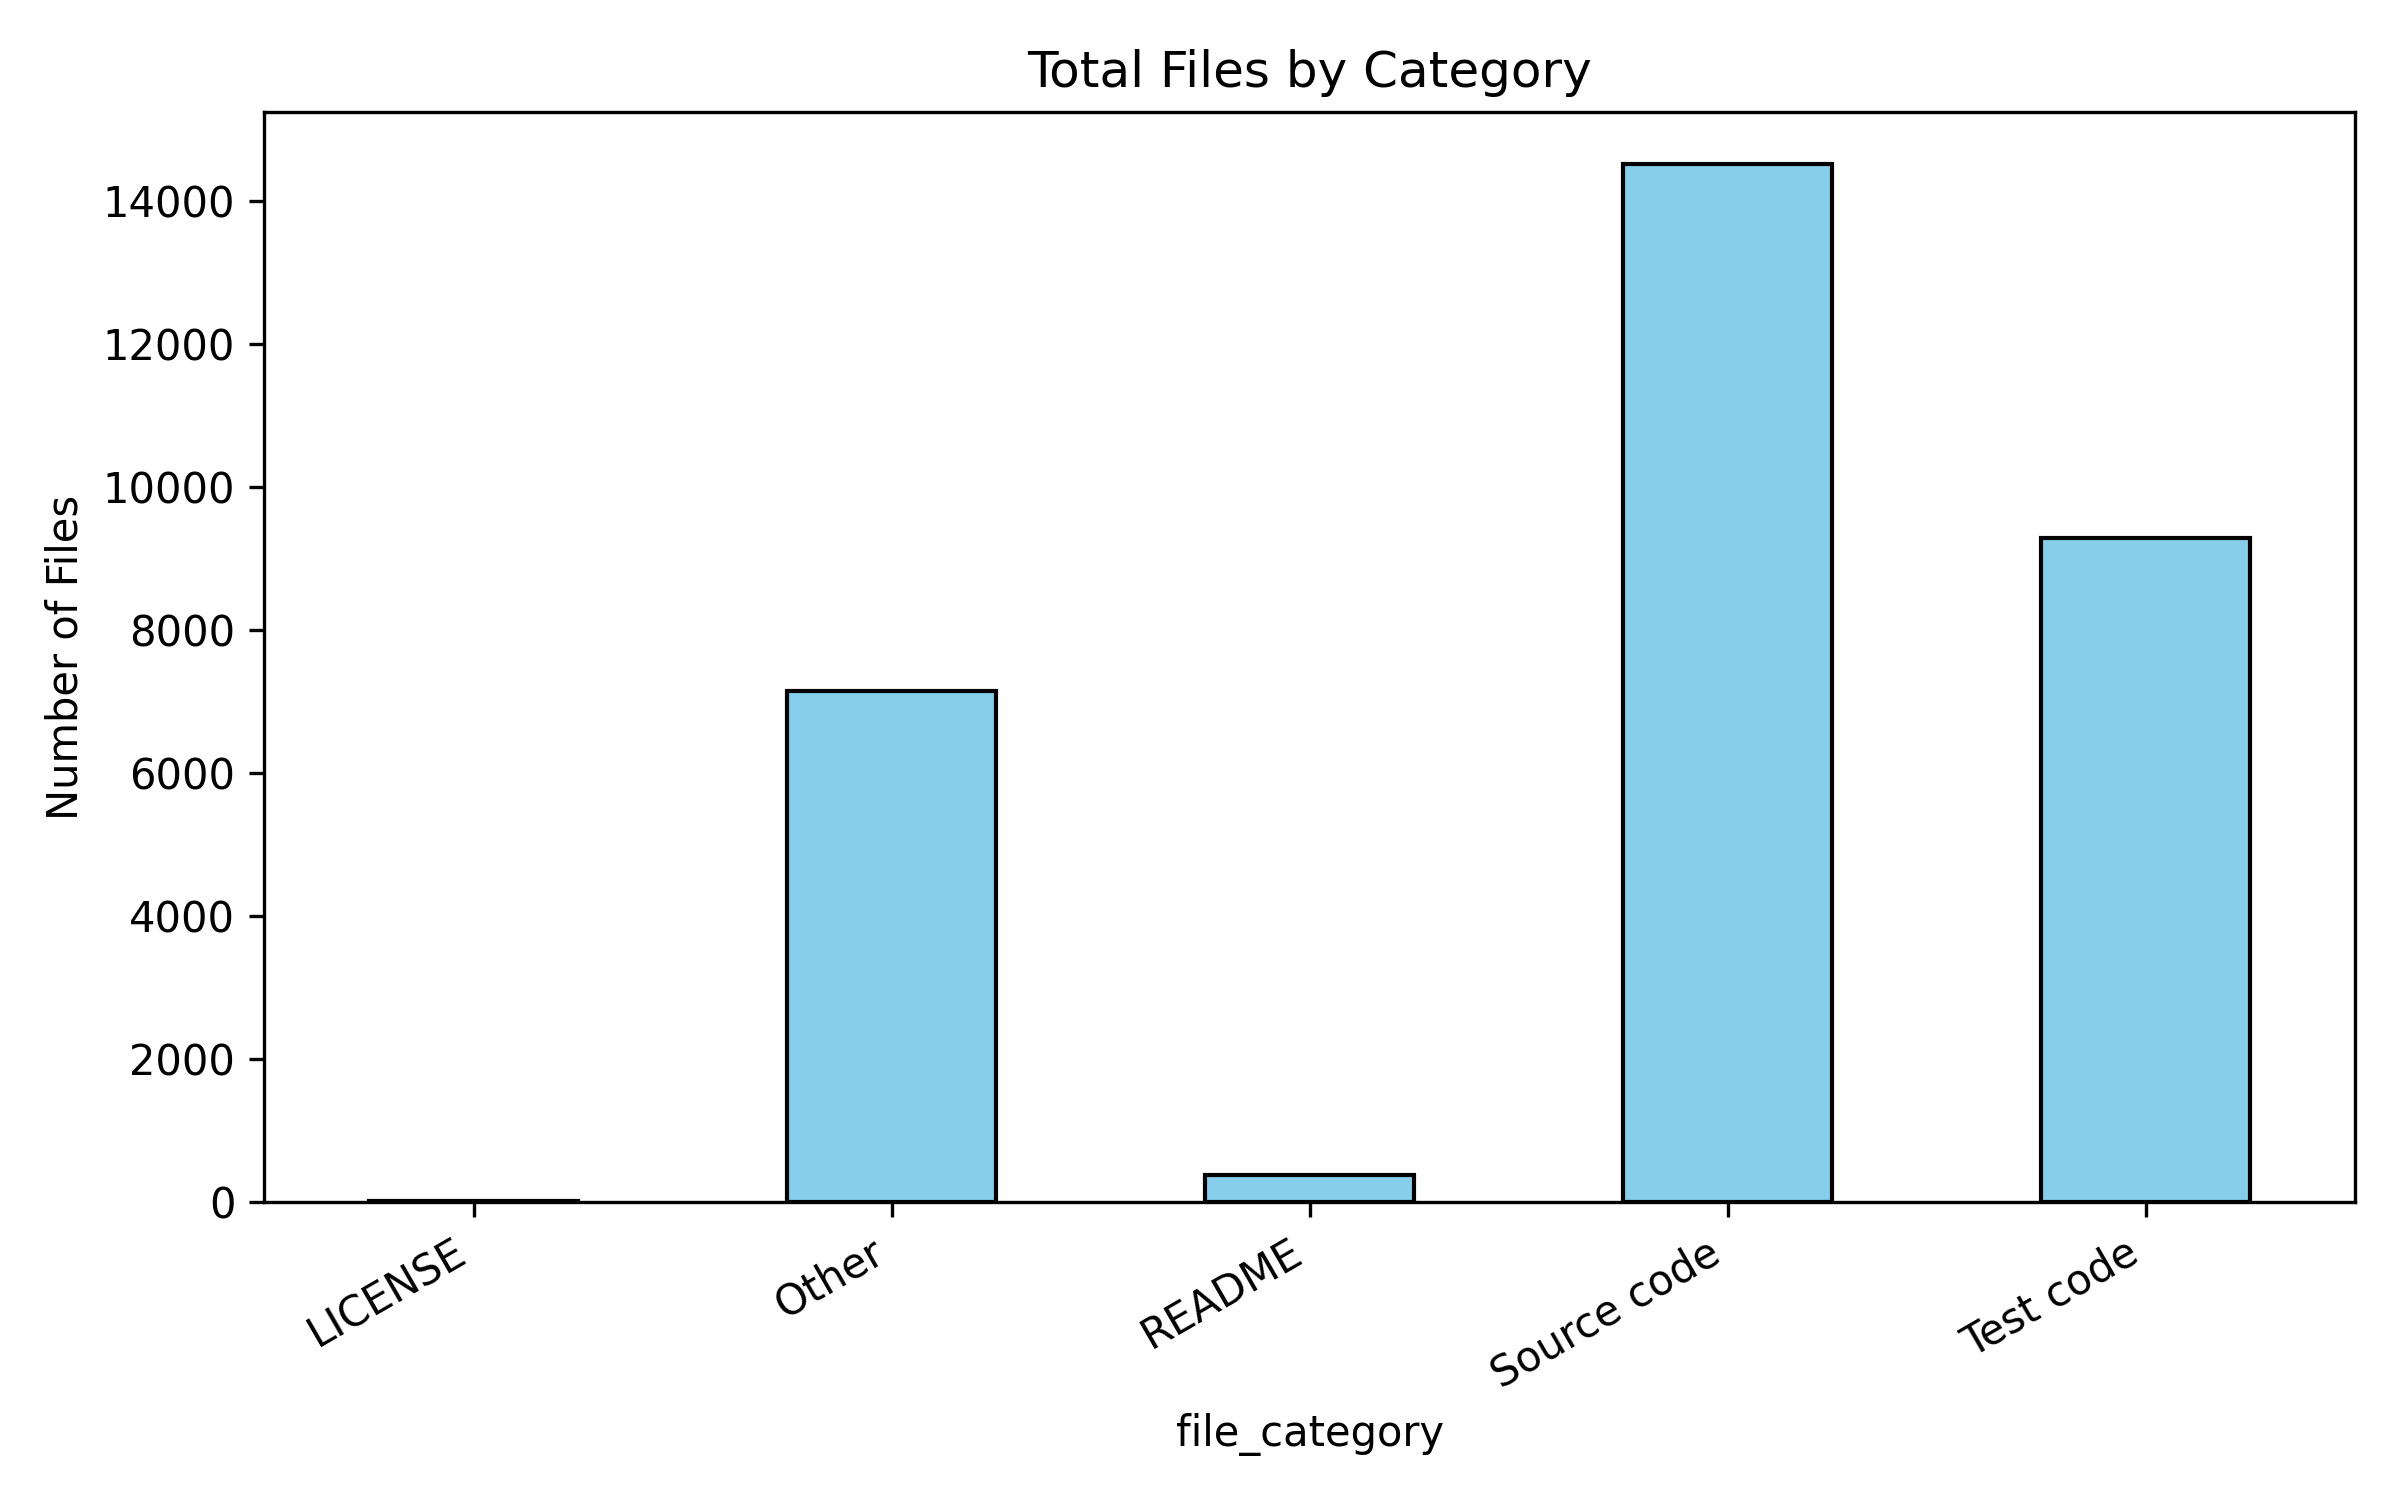
\includegraphics[width=0.8\textwidth]{/Users/tejasmacipad/Desktop/Third_year/STT/lab4report/total_files_by_category.png}
                \caption{Bar chart showing the total number of files per file category.}
            \end{figure}

            \item \textbf{Mismatches by File Category:}  
            \begin{figure}[!h]
                \centering
                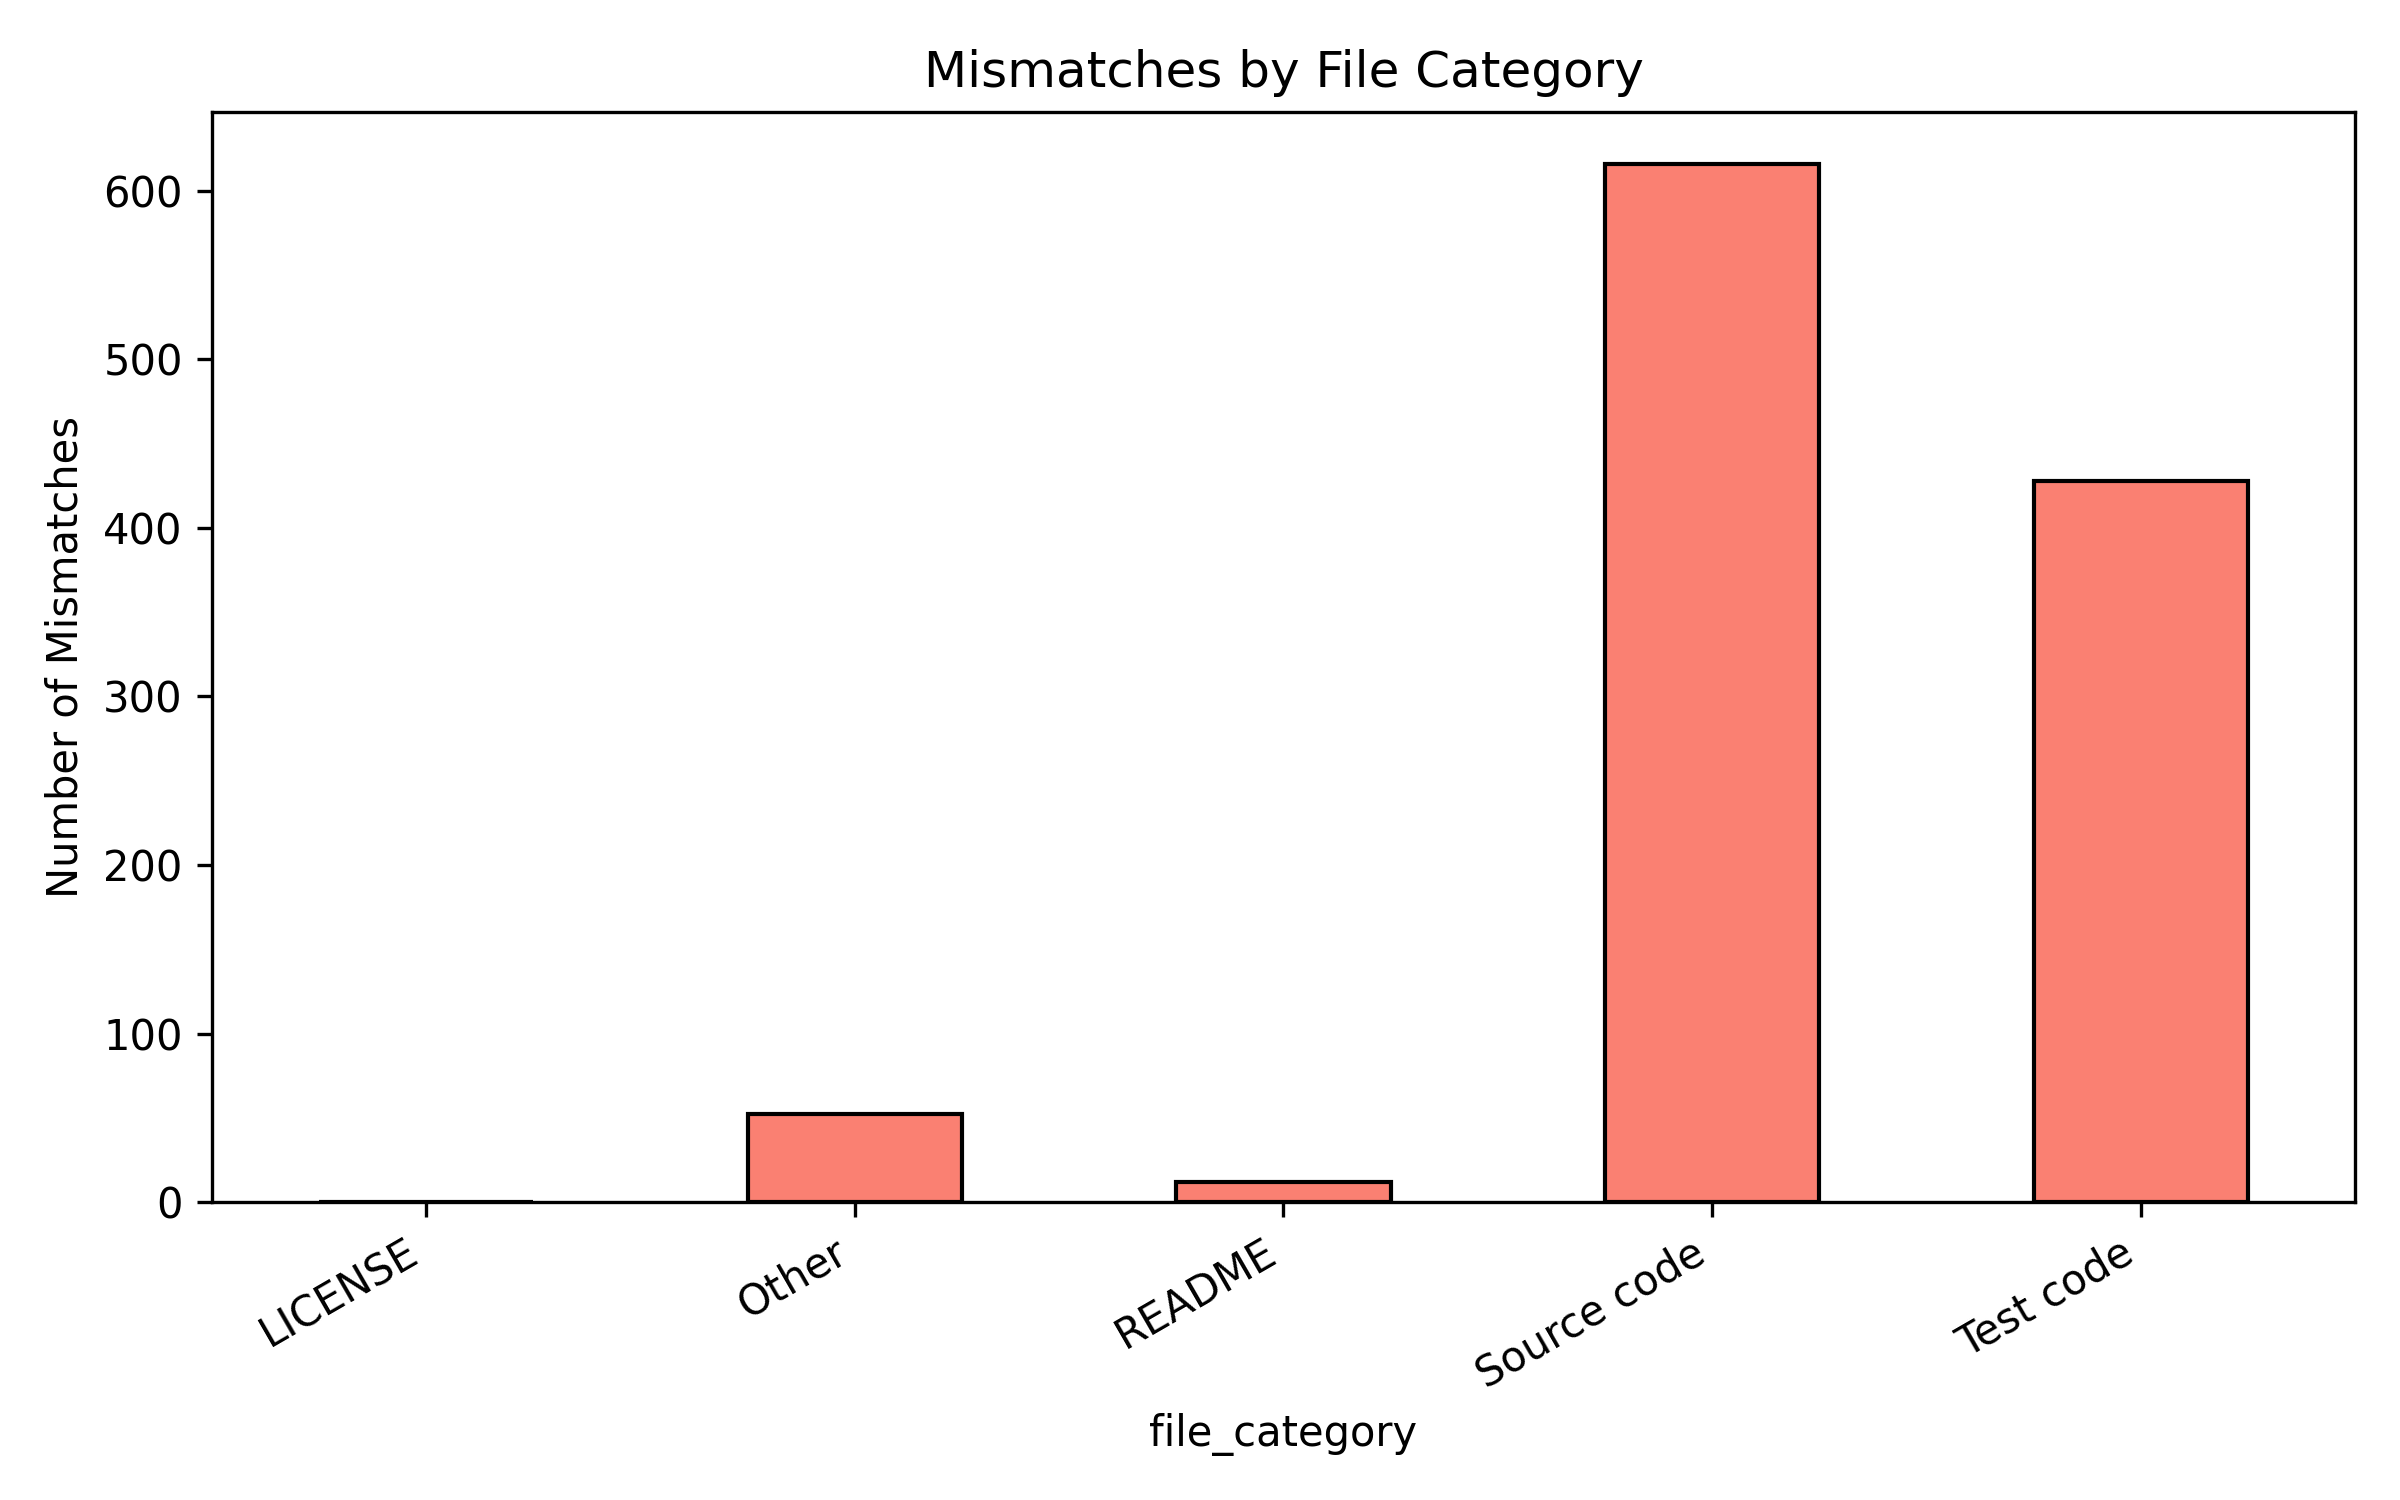
\includegraphics[width=0.8\textwidth]{/Users/tejasmacipad/Desktop/Third_year/STT/lab4report/mismatches_by_category.png}
                \caption{Bar chart showing the number of mismatches for each file category.}
            \end{figure}

            \item \textbf{Mismatch Percentage by File Category:}  
            \begin{figure}[!h]
                \centering
                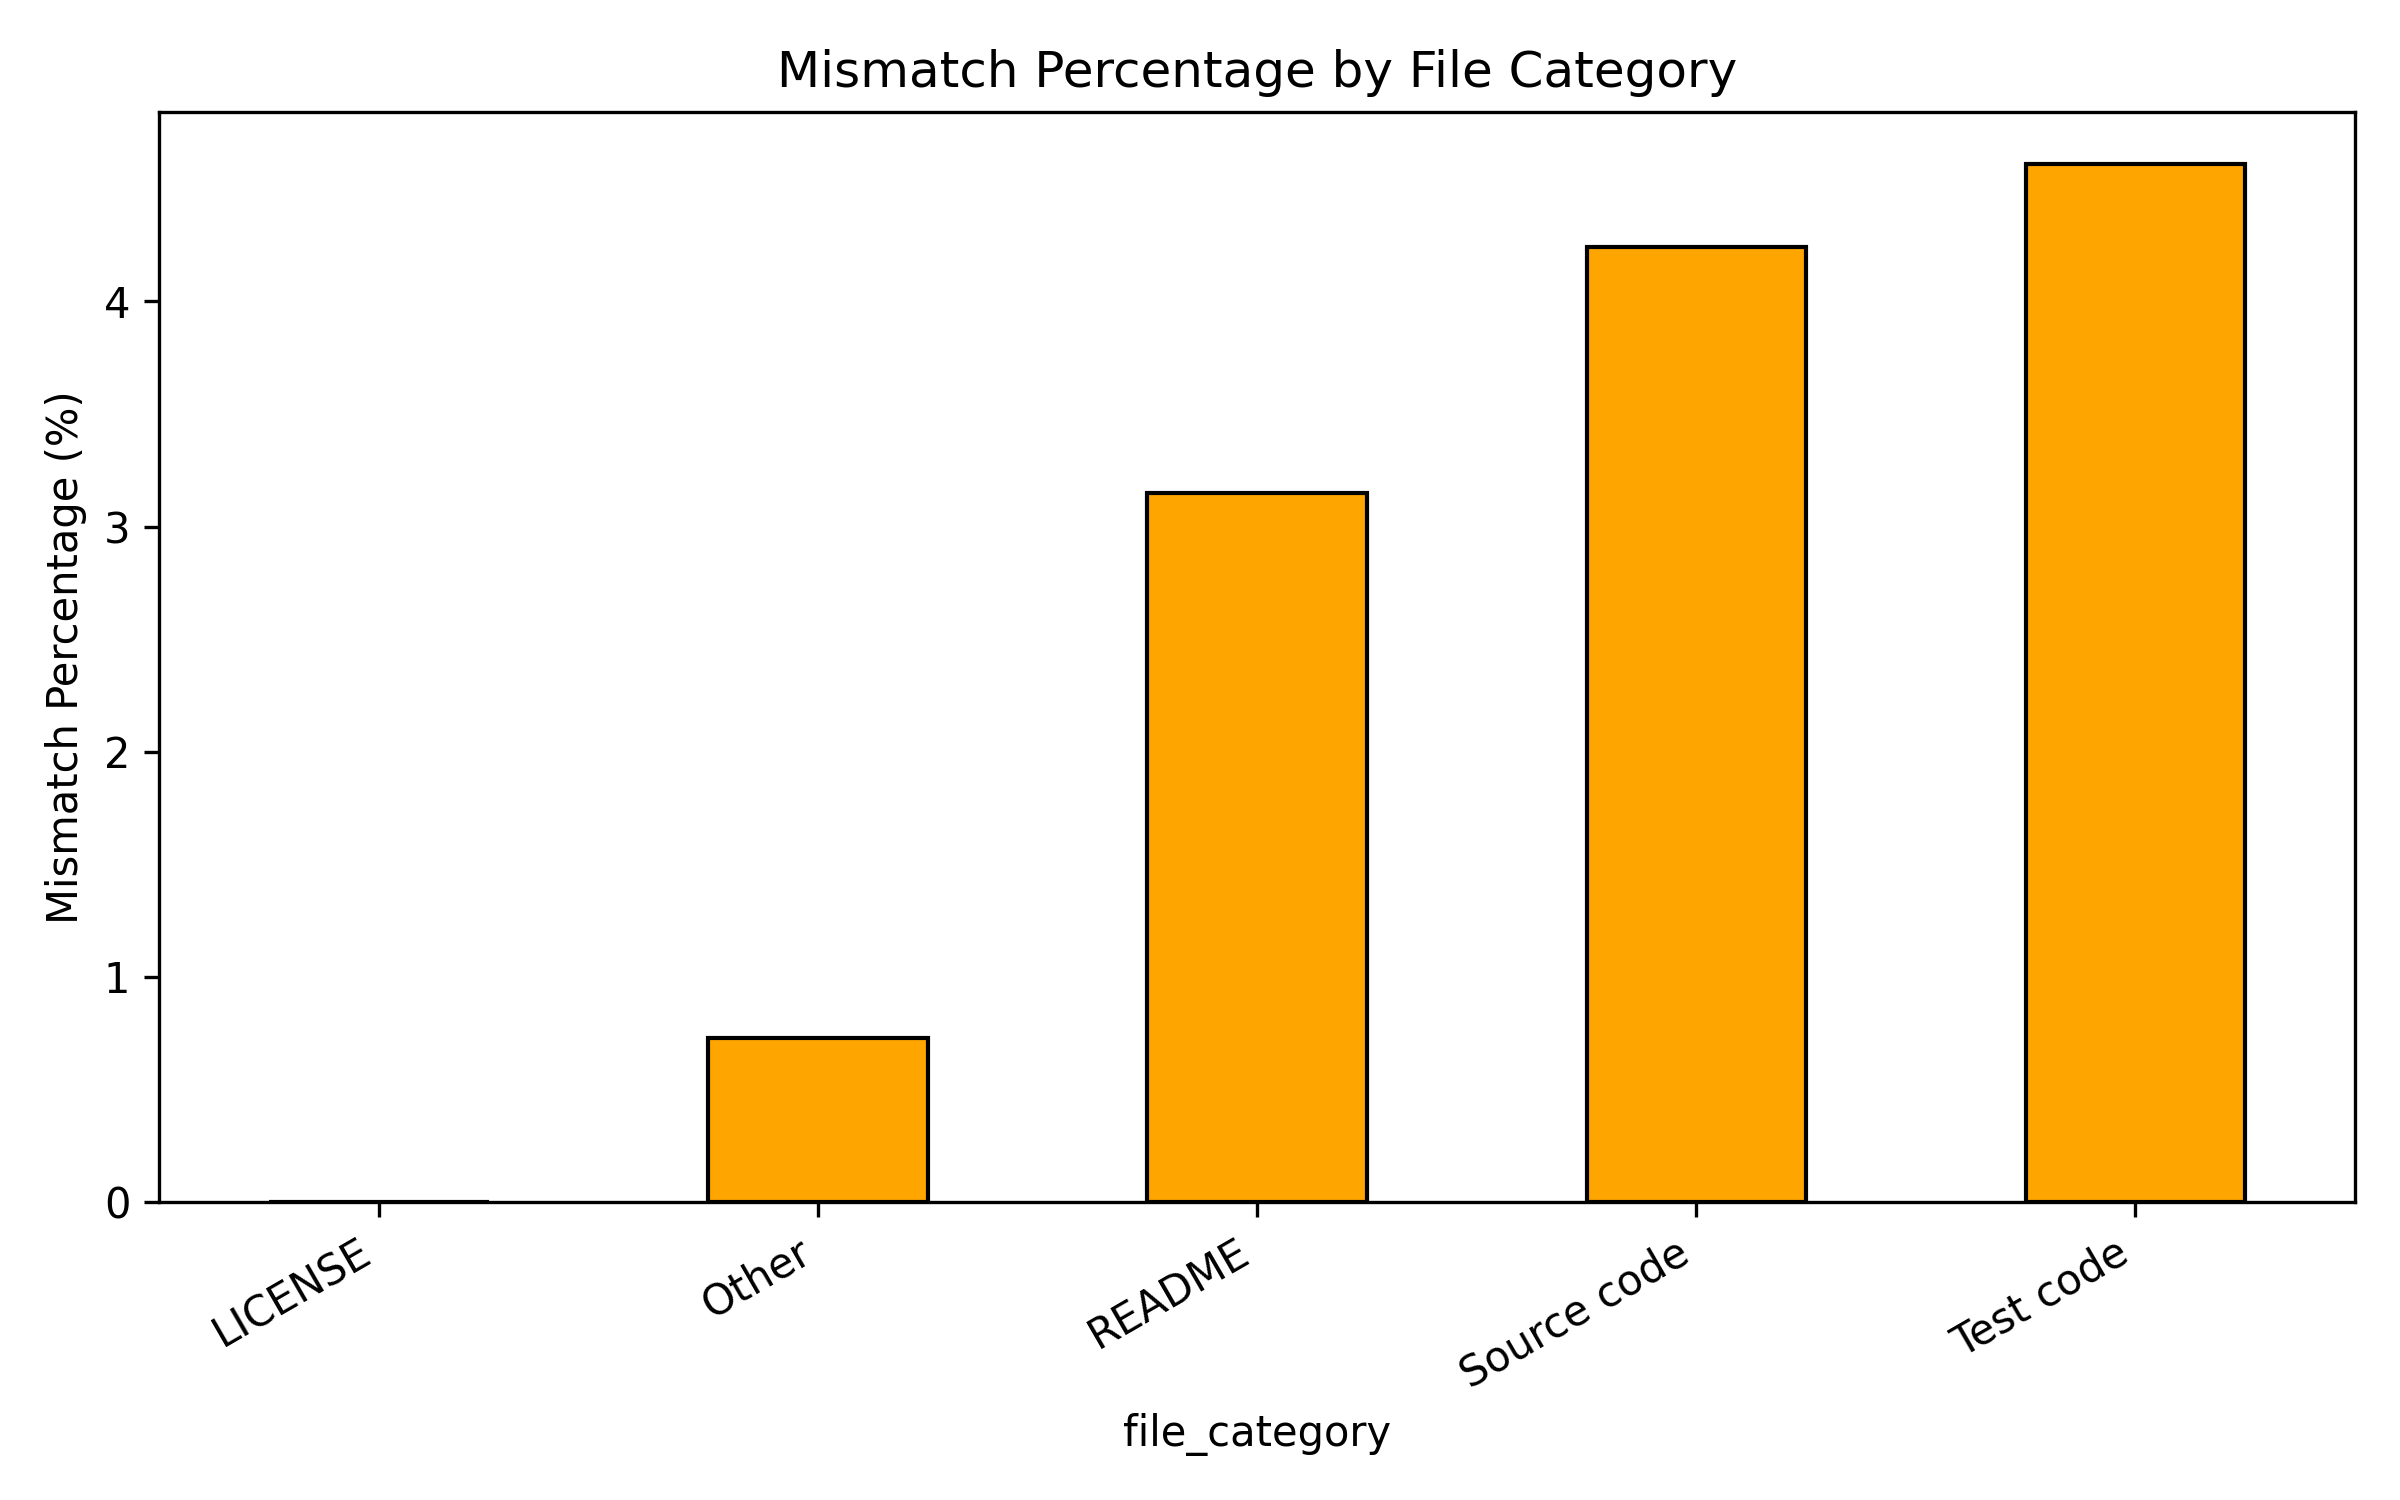
\includegraphics[width=0.8\textwidth]{/Users/tejasmacipad/Desktop/Third_year/STT/lab4report/mismatch_percentage_by_category.png}
                \caption{Bar chart displaying the mismatch percentage per file category.}
            \end{figure}

            \item \textbf{Top 10 File Extensions by Mismatch Percentage:}  
            \begin{figure}[!h]
                \centering
                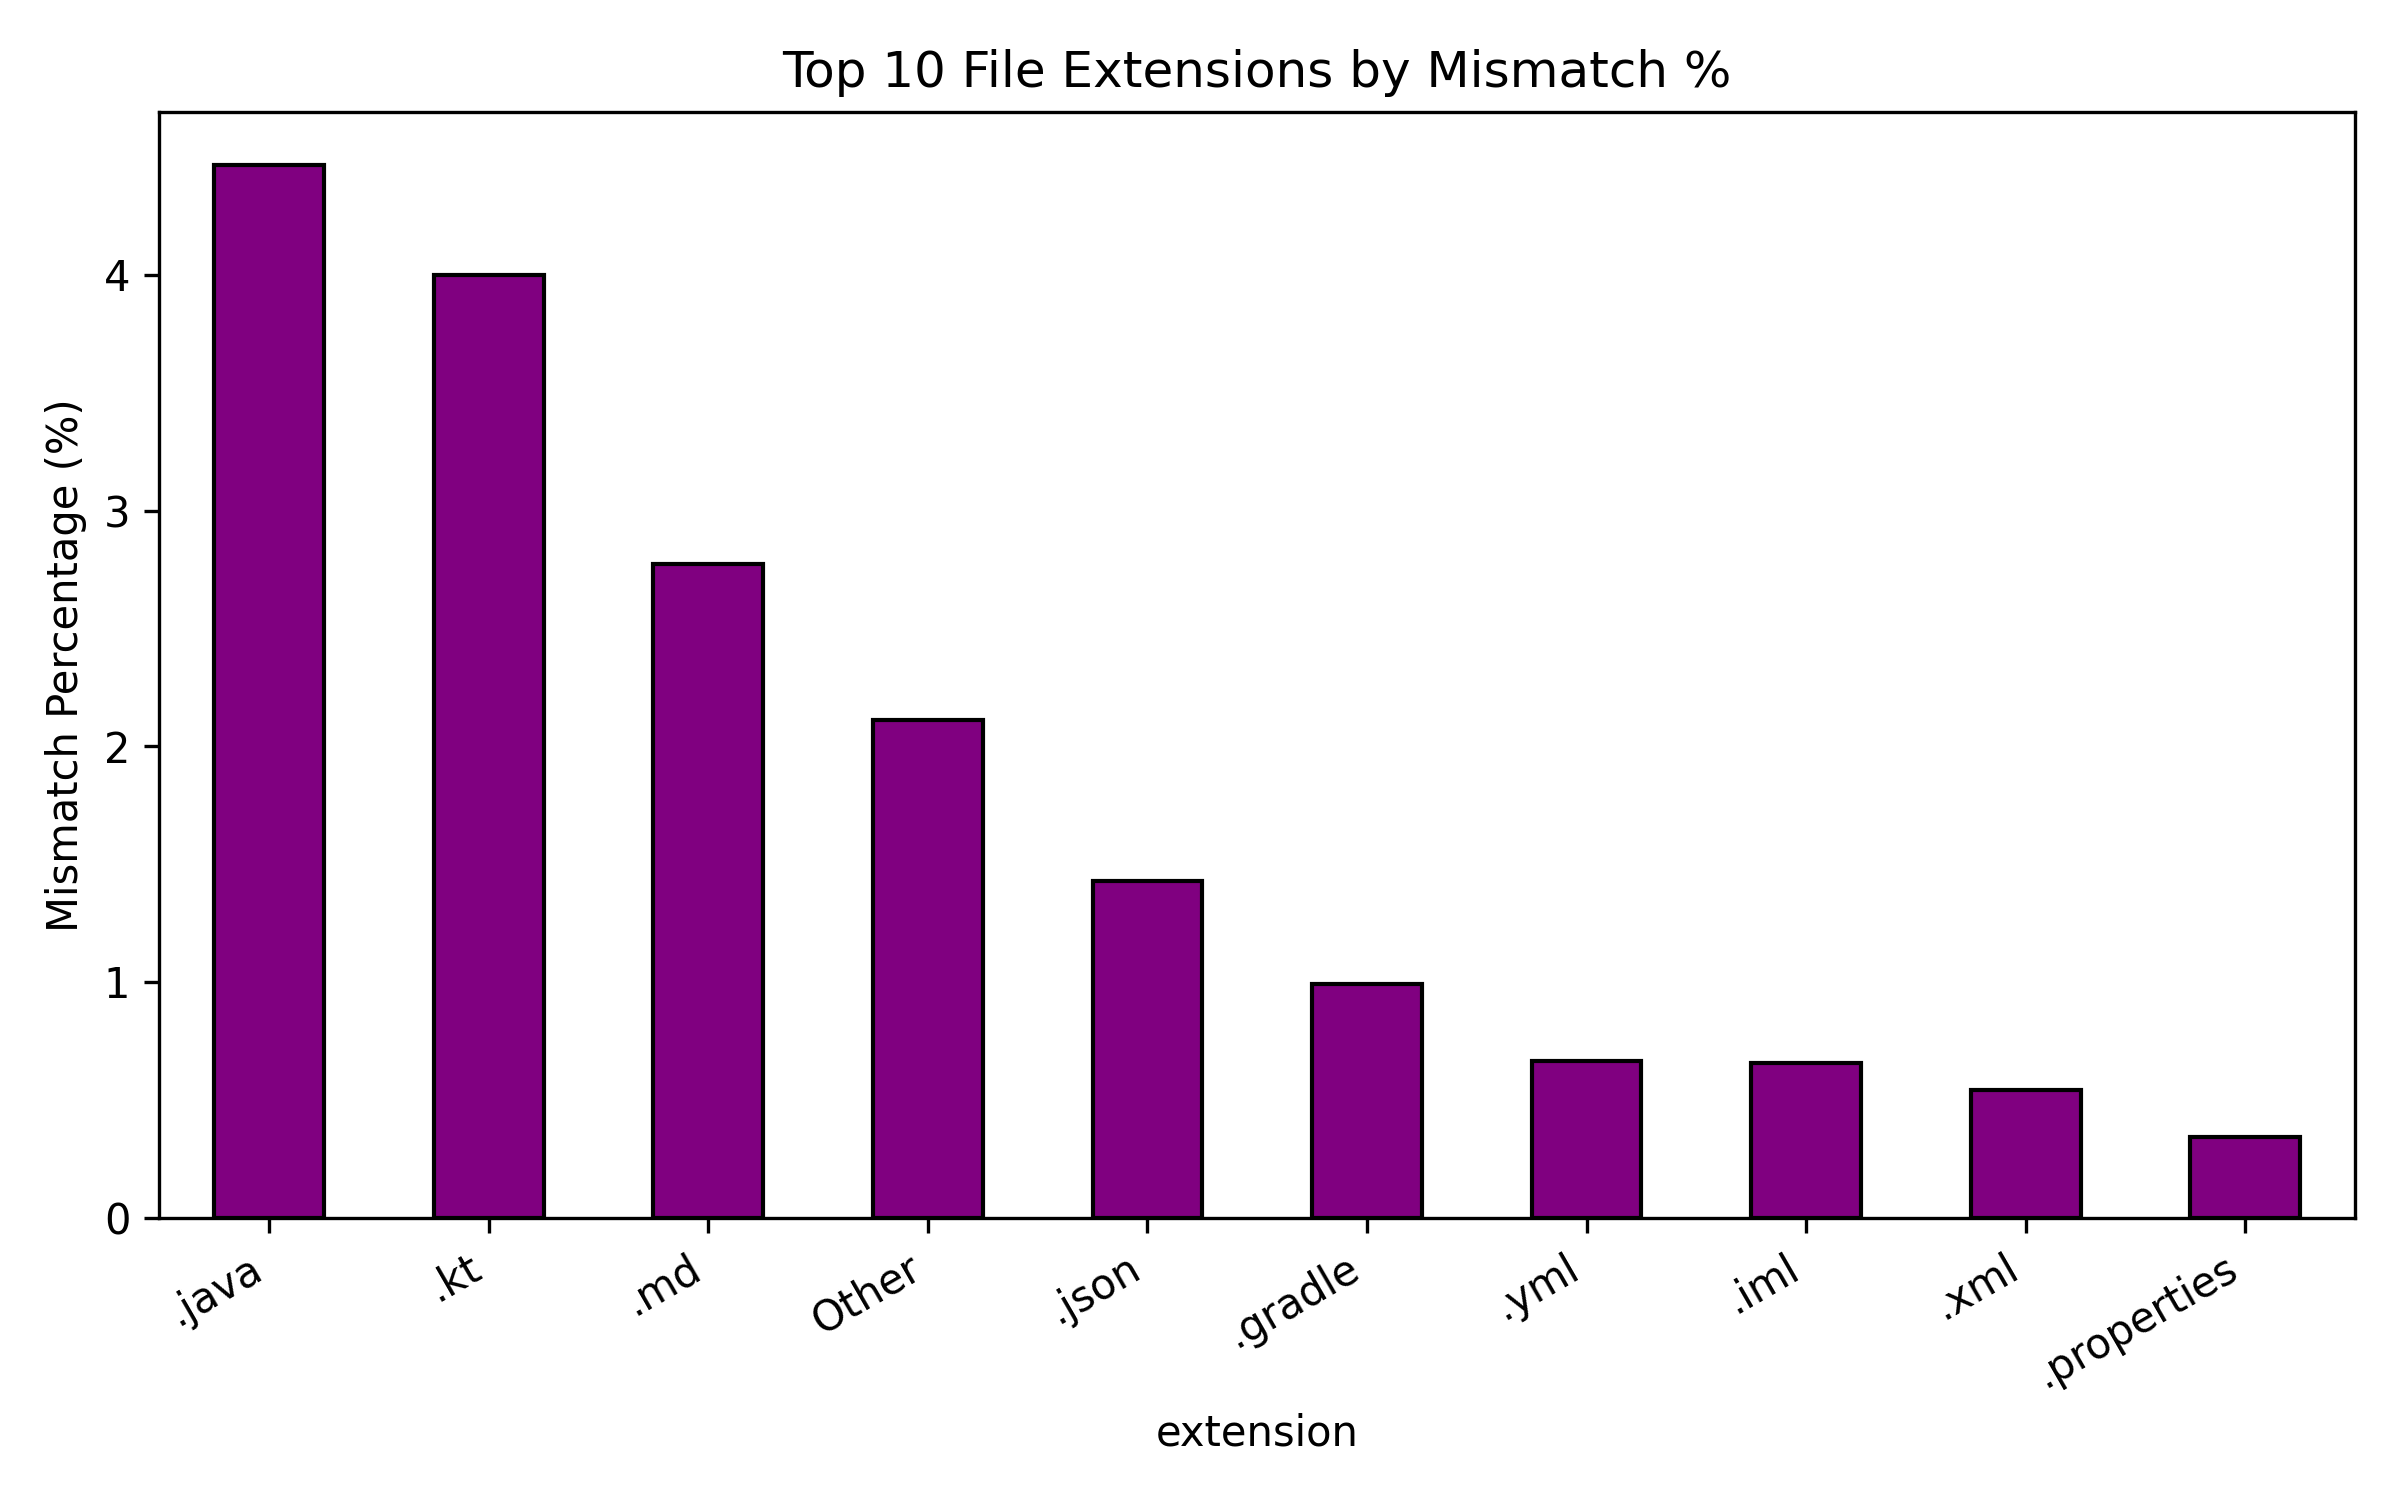
\includegraphics[width=0.8\textwidth]{/Users/tejasmacipad/Desktop/Third_year/STT/lab4report/top_extensions_mismatch.png}
                \caption{Bar chart highlighting the top 10 file extensions with the highest mismatch percentages.}
            \end{figure}

            \item \textbf{Mismatch Percentage by Repository:}  
            \begin{figure}[!h]
                \centering
                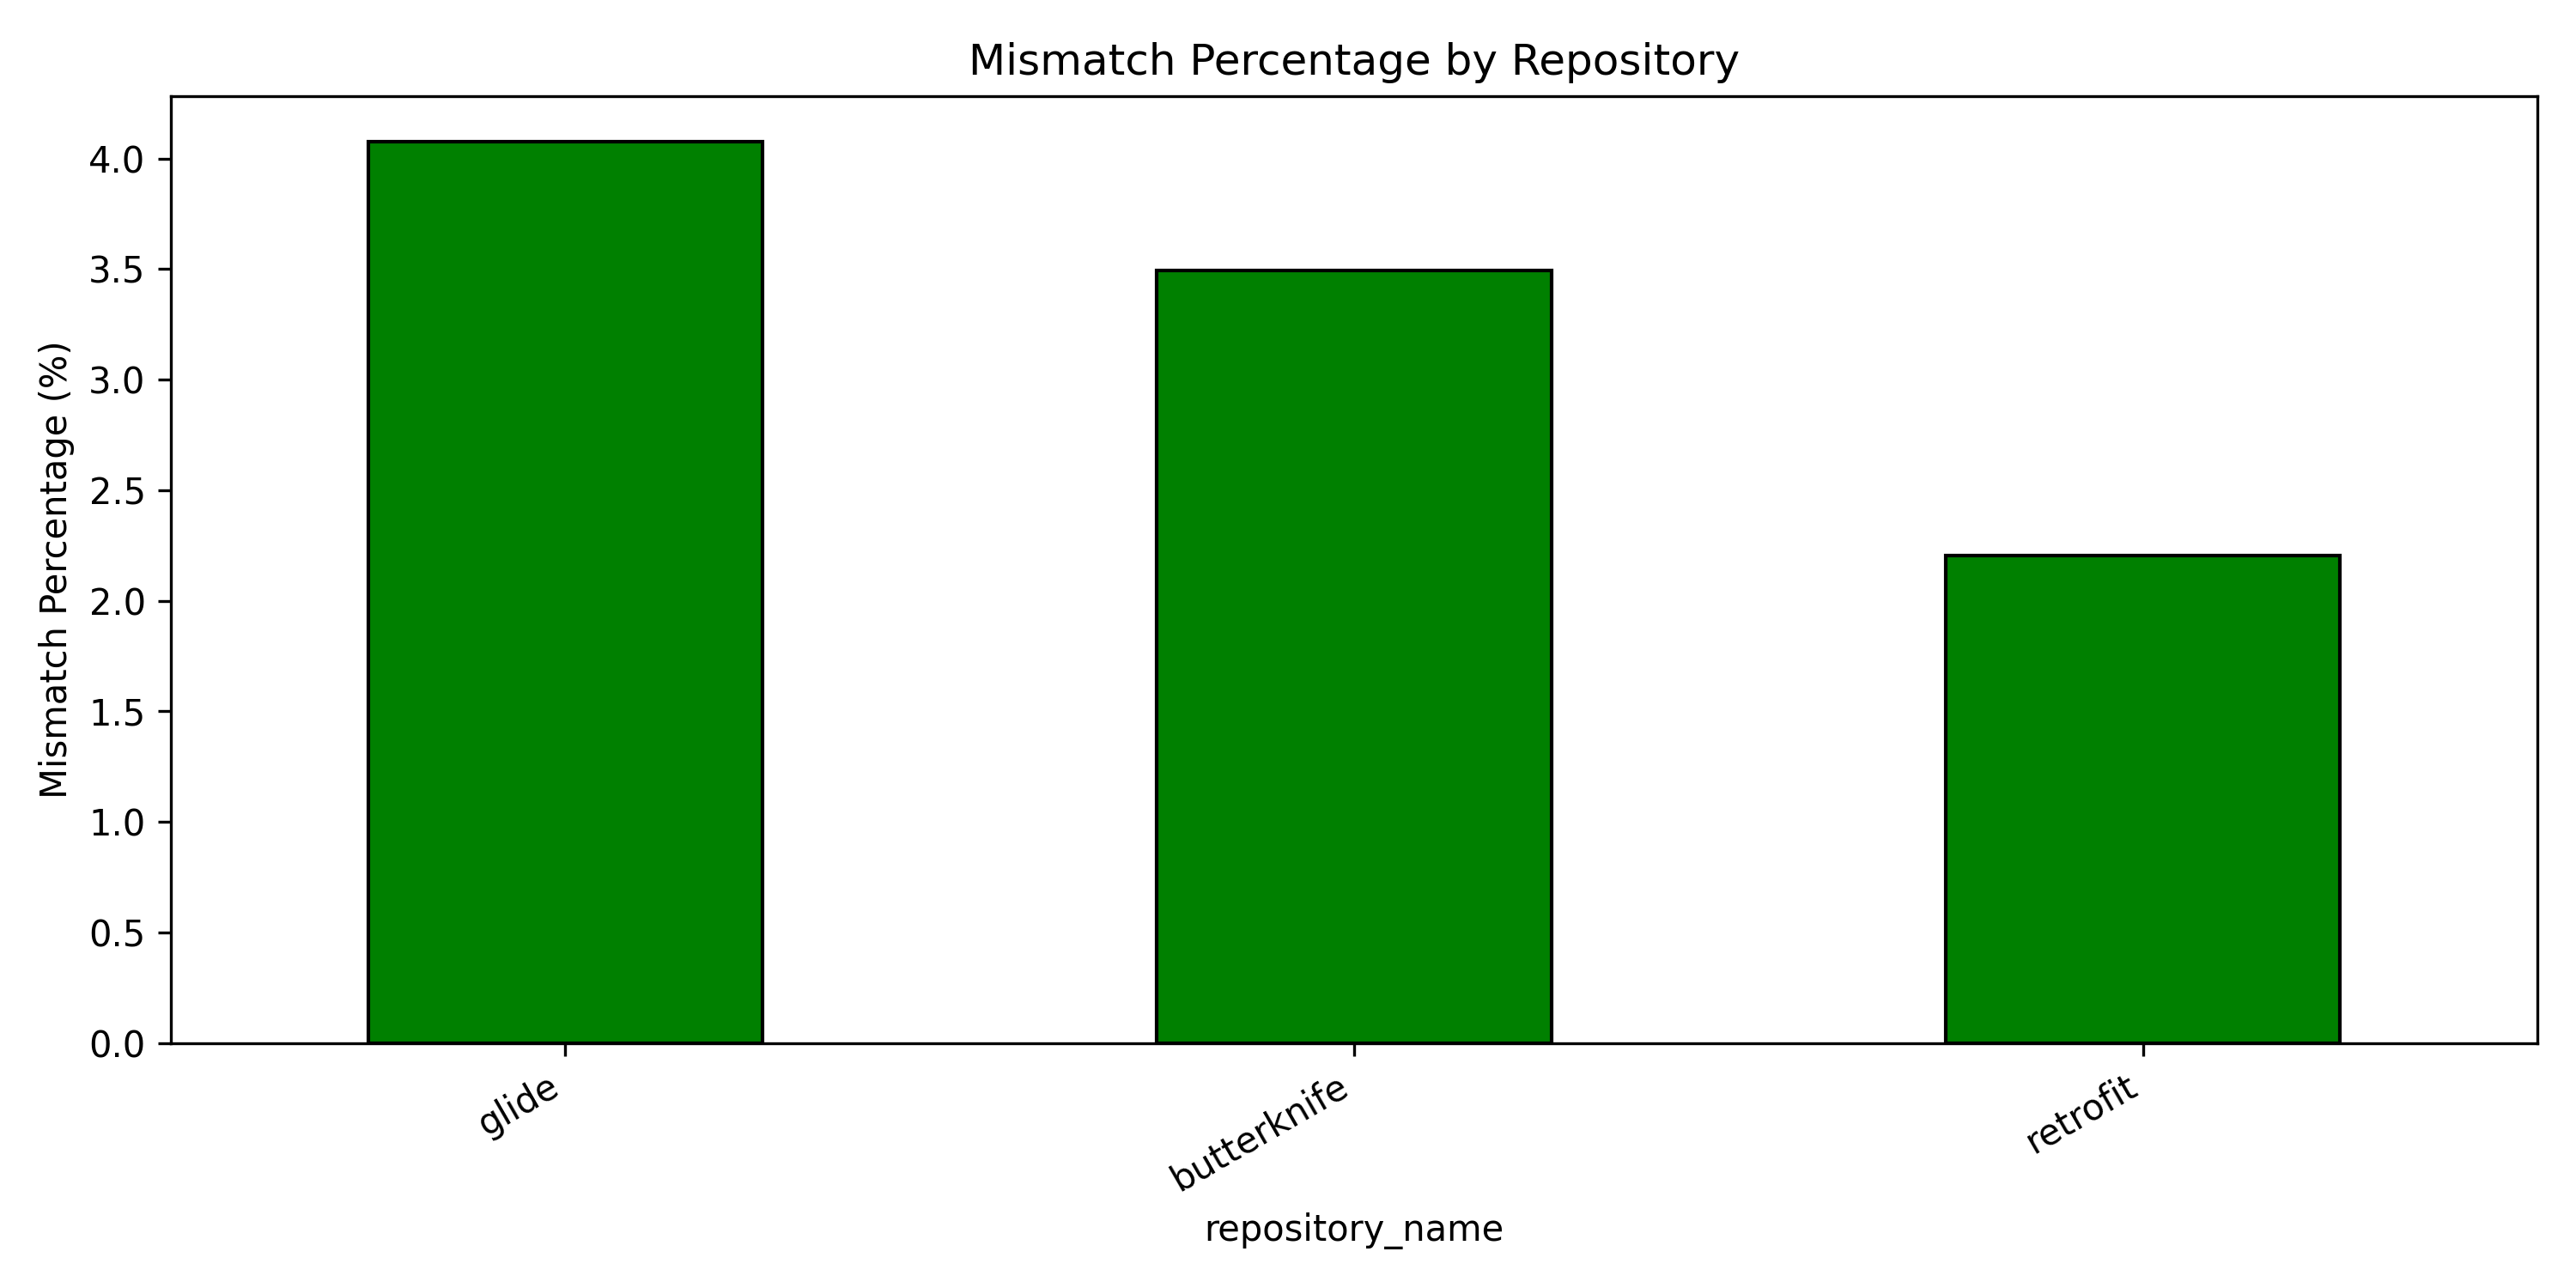
\includegraphics[width=0.8\textwidth]{/Users/tejasmacipad/Desktop/Third_year/STT/lab4report/repo_mismatch_percentage.png}
                \caption{Bar chart showing mismatch percentages across repositories.}
            \end{figure}

            \item \textbf{Distribution of Mismatches per Commit:}  
            \begin{figure}[!h]
                \centering
                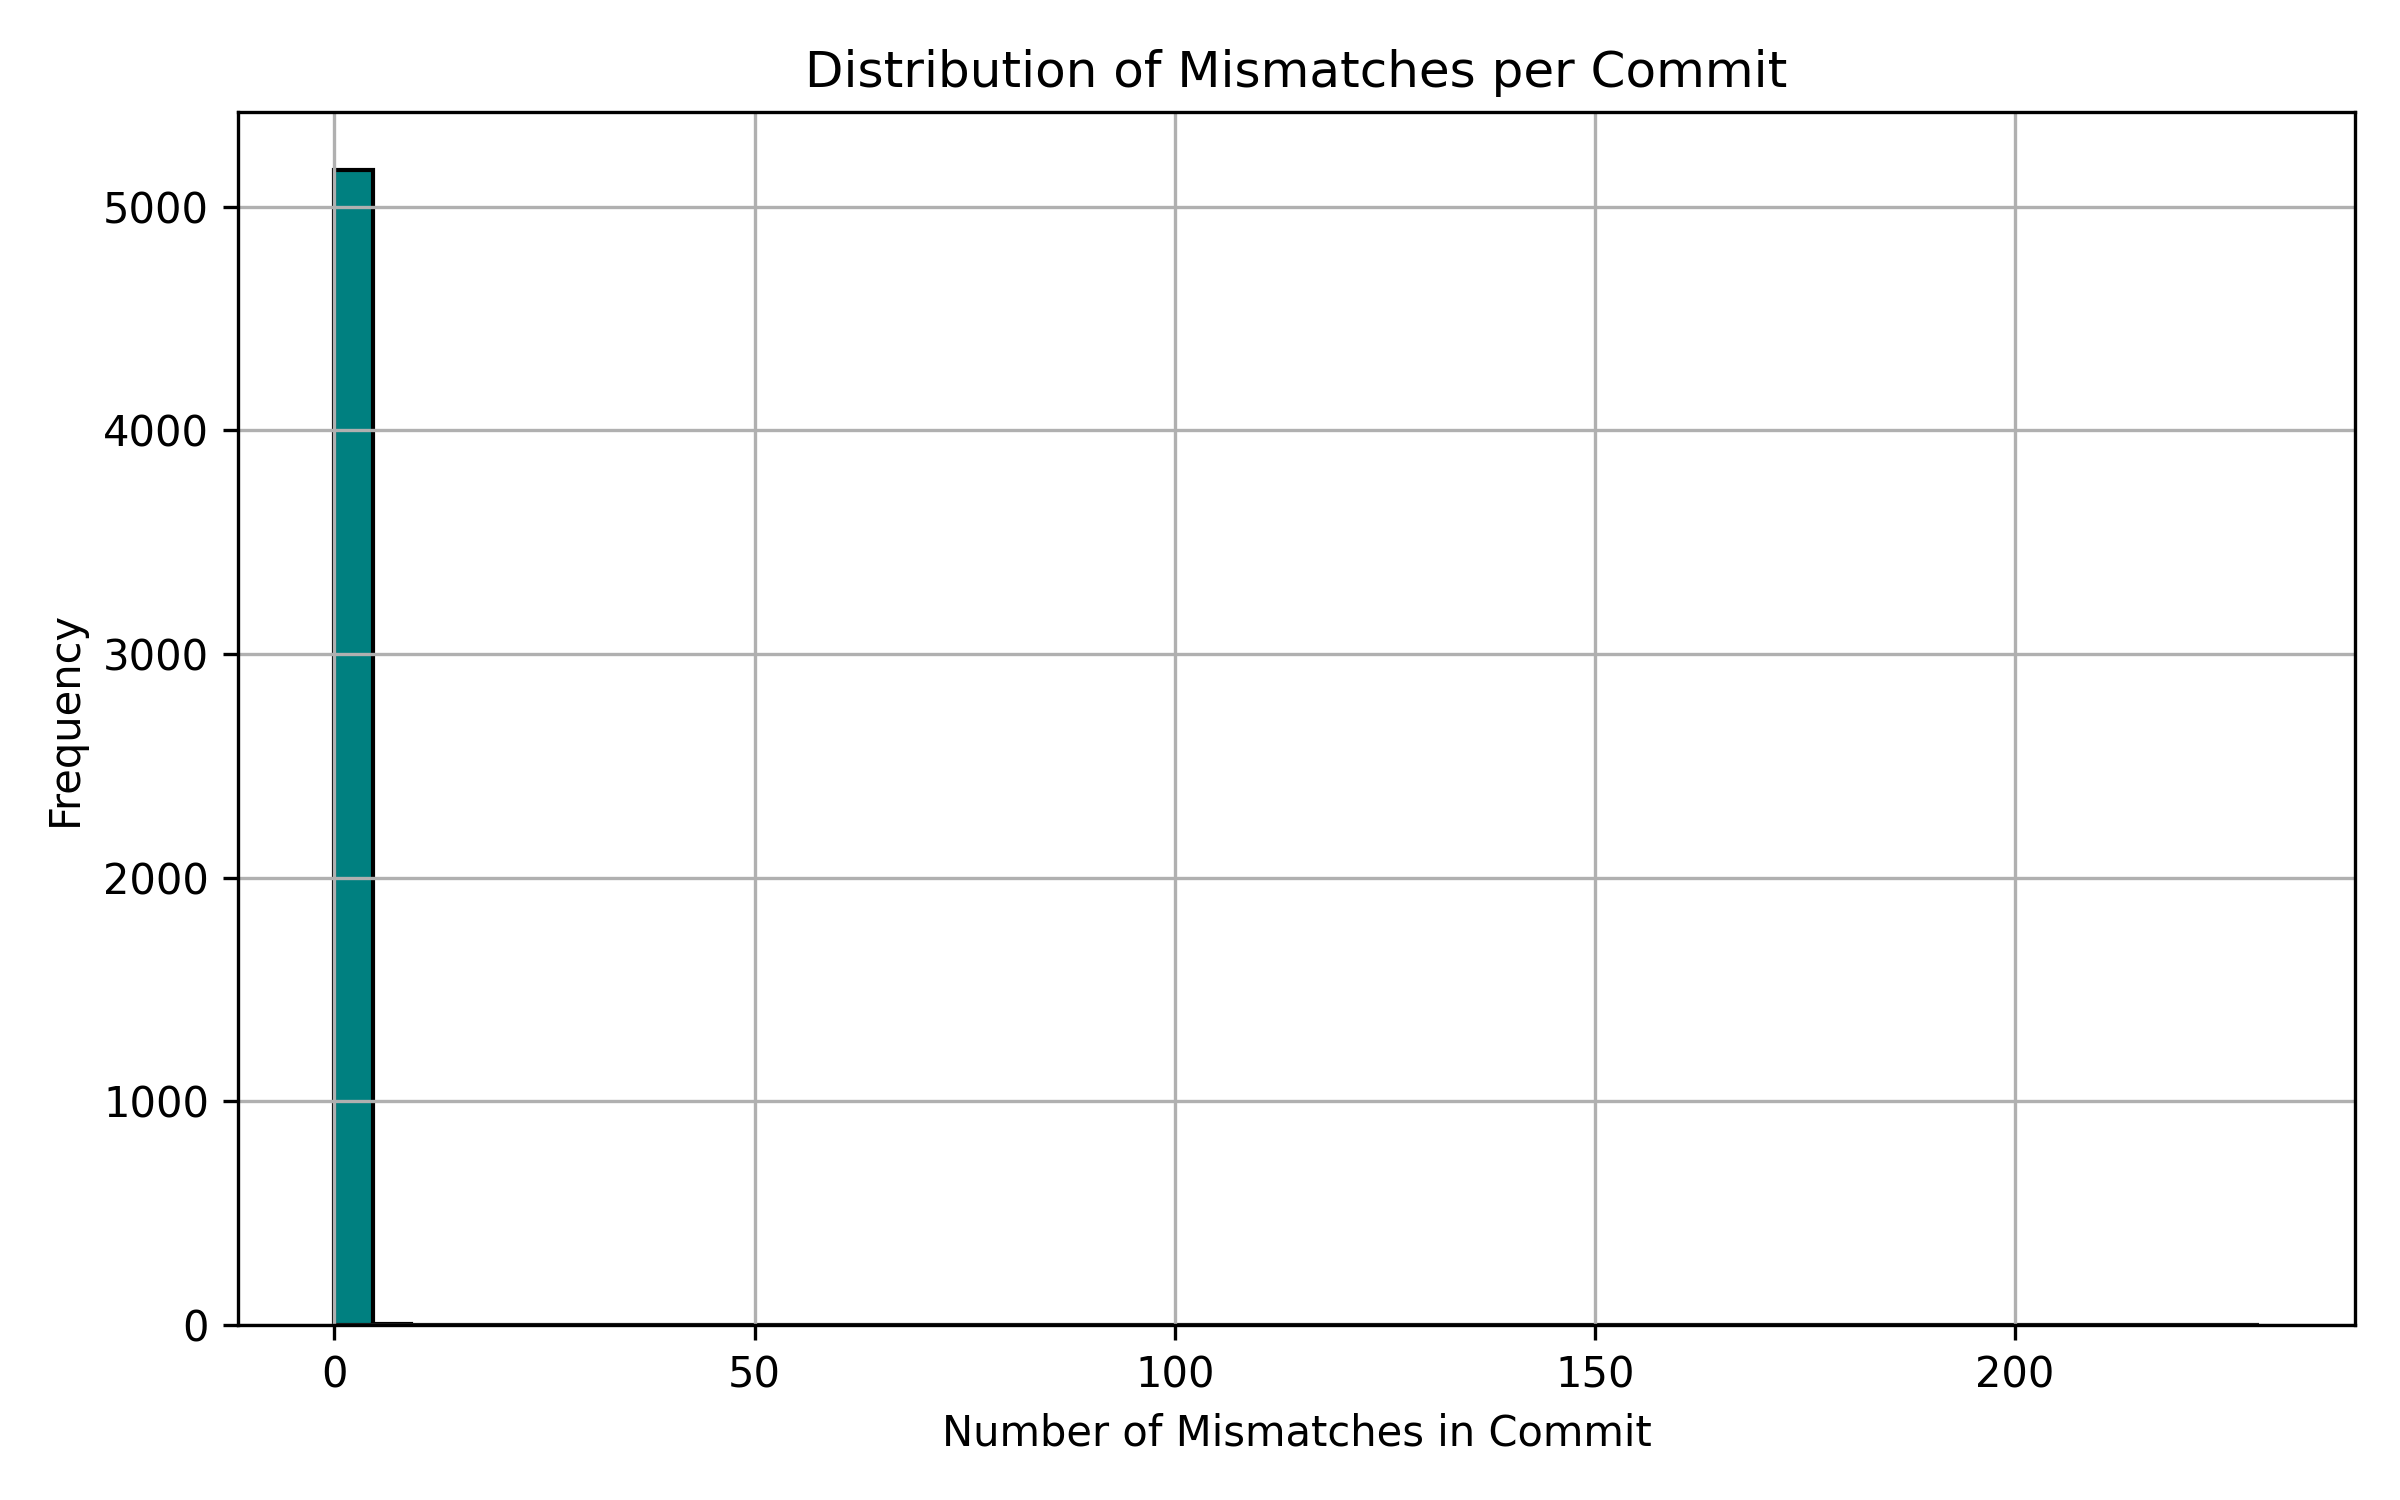
\includegraphics[width=0.8\textwidth]{/Users/tejasmacipad/Desktop/Third_year/STT/lab4report/distribution_mismatches_commit.png}
                \caption{Histogram illustrating the distribution of mismatches per commit.}
            \end{figure}

            \item \textbf{Top 10 Commits by Number of Mismatches:}  
            \begin{figure}[!h]
                \centering
                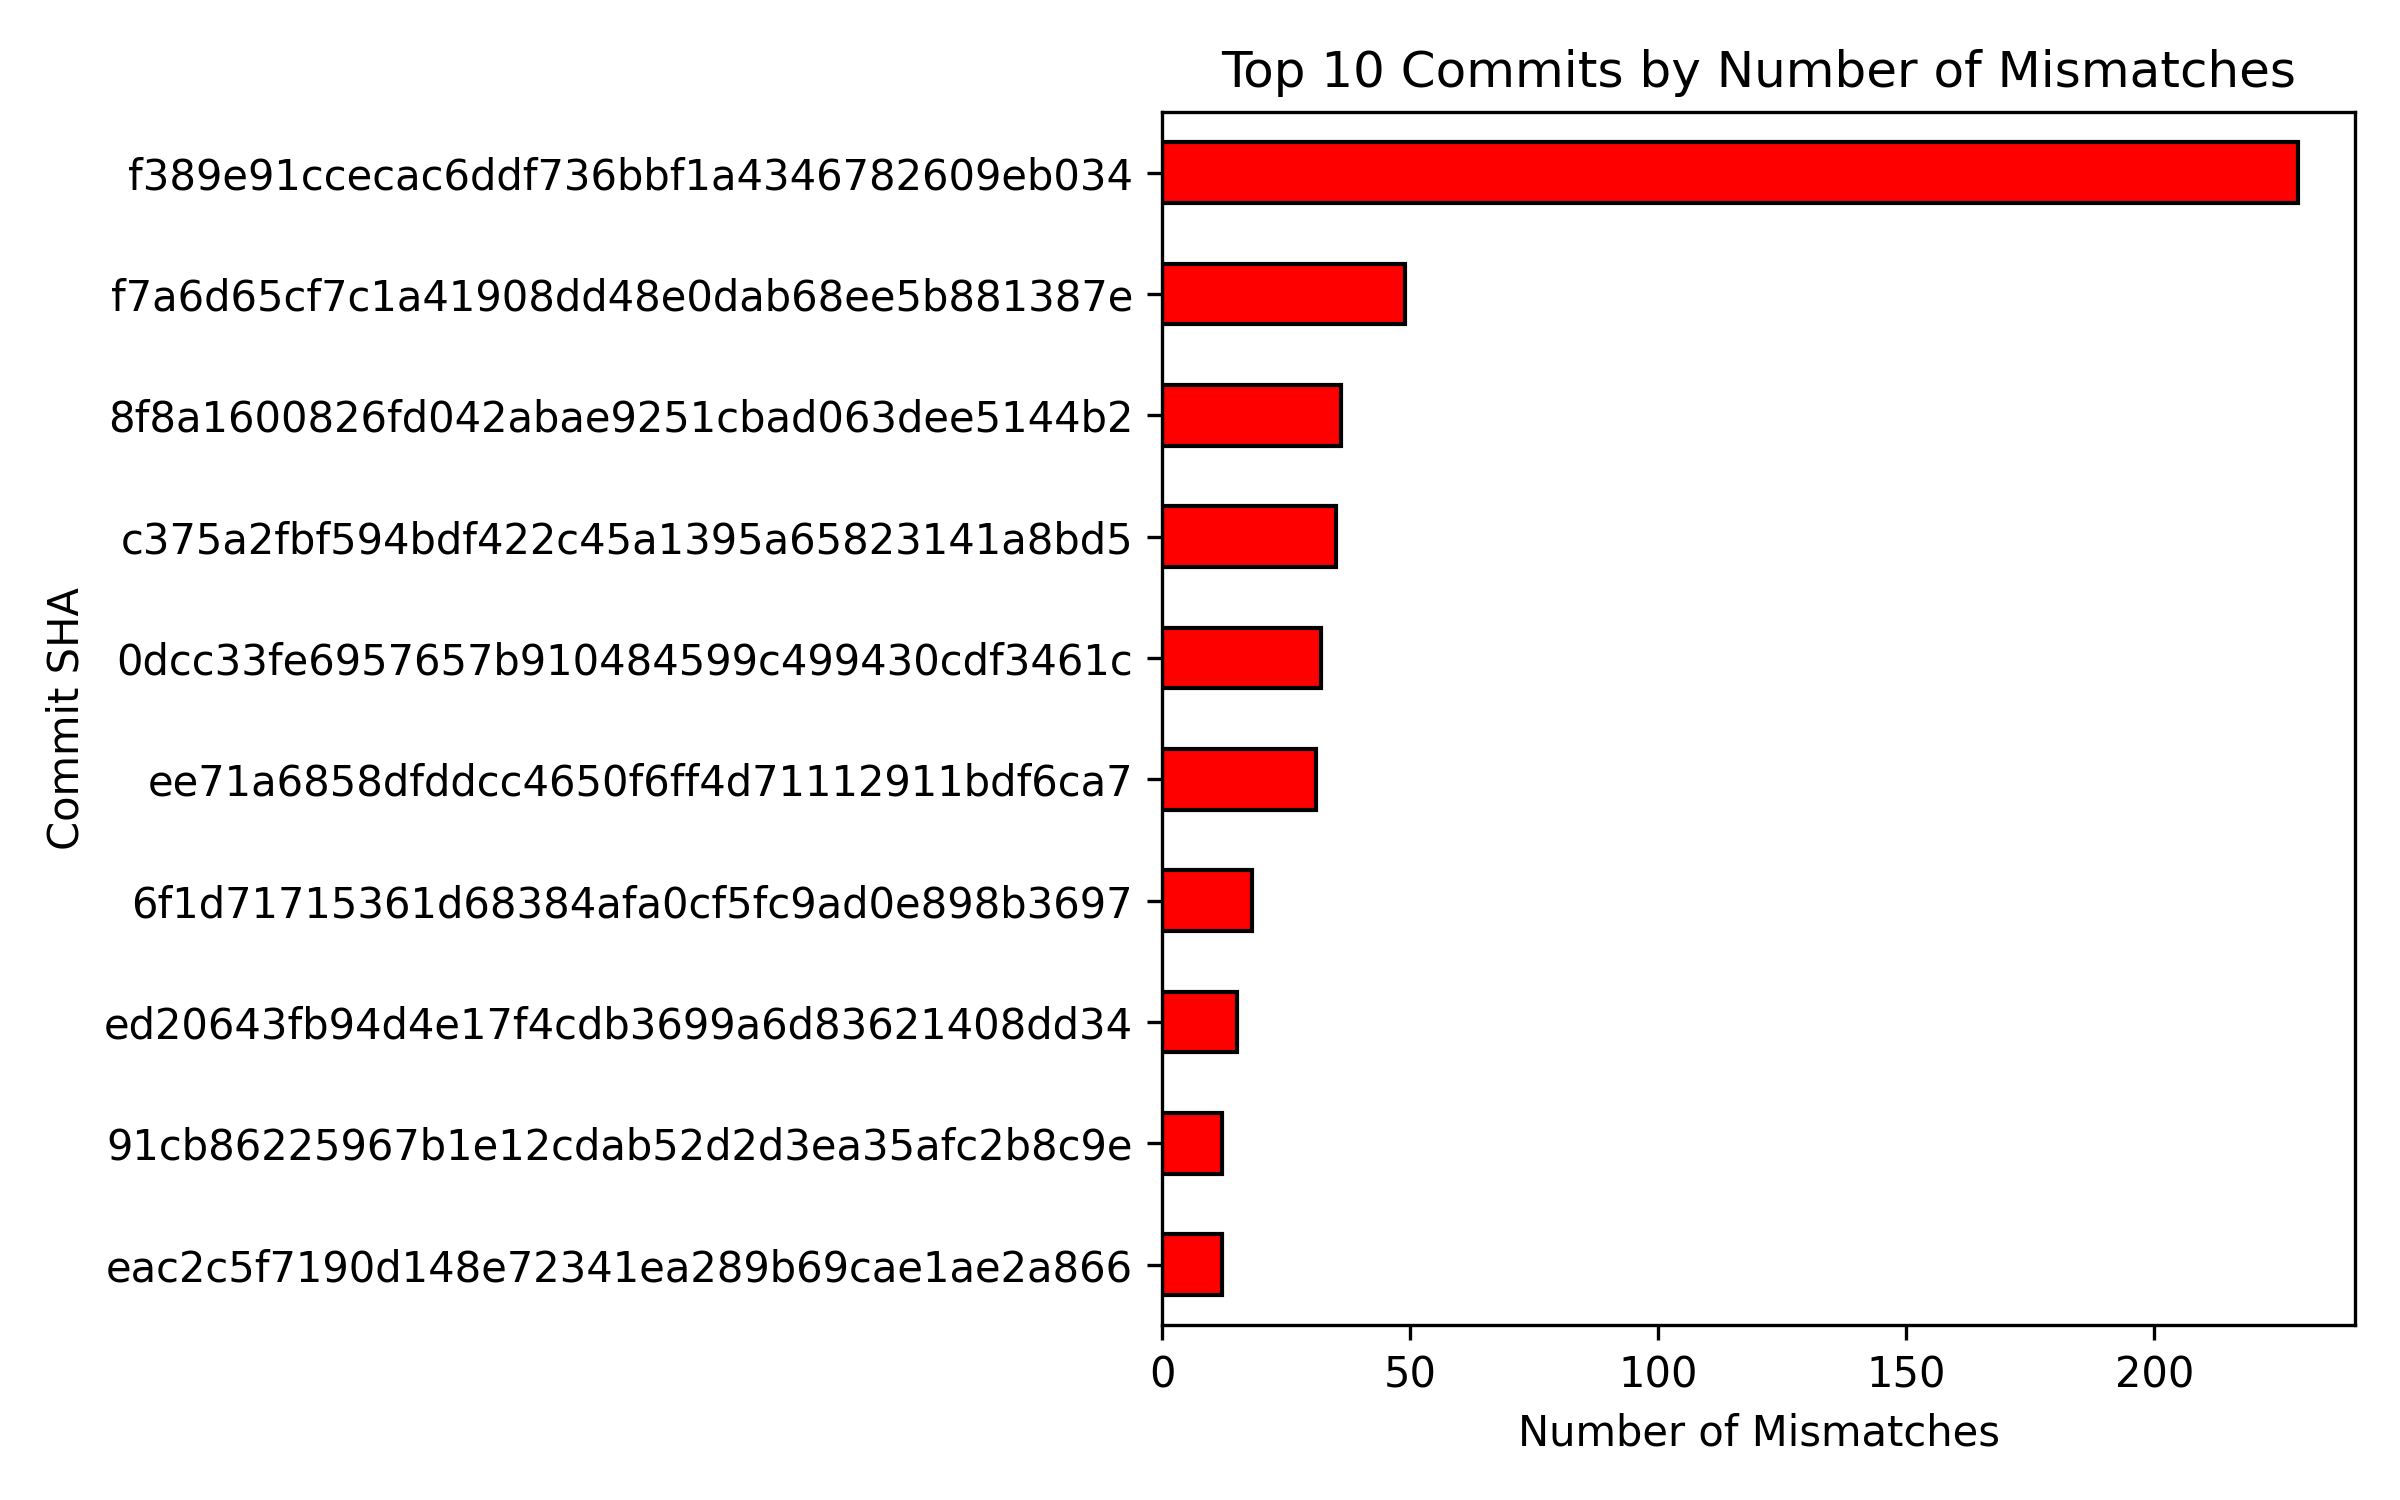
\includegraphics[width=0.8\textwidth]{/Users/tejasmacipad/Desktop/Third_year/STT/lab4report/top_commits_mismatches.png}
                \caption{Horizontal bar chart displaying the top 10 commits responsible for the most mismatches.}
            \end{figure}
        \end{itemize}
\end{enumerate}

These plots and statistics prove an understanding of the dataset's structure and the nature of the mismatches present.

\subsection*{Part F: Which algorithm performed better}
\begin{itemize}
    \item \texttt{Metric Definition} -- We can define multiple metrics to evaluate the performance of the algorithms, such as number of mismatches, percentage of mismatches, runtime efficiency (Compute required).
    \item \texttt{Run Model to find various metrics} -- Execute the models on the dataset to obtain the defined metrics for each algorithm.
    \item \texttt{Conclusive analysis} -- Just based on the results on a single repository, we cannot conclude which algorithm is better. However, based on the results from all three repositories, we can perform Statistical tests to compare the algorithms more rigorously to prove\/disprove any hypothesis.
    \item \texttt{Script to run these tests} -- Automating the script to report the result which includes to run the model to get metrics, run statistical tests(optional), and report the one which scores better.
\end{itemize}



\end{document}